\newpage
\section{Aufgabe 1}

\subsection{Aufgabenstellung}
Sie haben in den vorhergehenden Praktika eigene Verteilte Anwendungen entwickelt, die Sie nun analysieren sollen.\\\\Gehen Sie wie folgt vor:

\begin{enumerate}[label=(\alph*)]
	\item Starten Sie die Wireshark-Software auf Ihrem Rechner und machen Sie sich mit den Möglichkeiten der Aufzeichnung des Netzwerkverkehrs und der detaillierten Anzeige der aufgezeichneten Abläufe vertraut.
	\item Realisieren Sie einen Filter für die Aufzeichnung des Netzwerkverkehrs, mit dem nur noch Frames mit TCP Segmenten mit der Portnummer 8999 aufgezeichnet werden.
	\item Starten Sie nun den Datentransfer, den Sie im vergangenen Praktikum implementiert haben (wahlweise die UDP- oder TCP-Variante).\\Stoppen Sie die Aufzeichnung sofort, wenn Client und Server beendet sind.
	\item Analysieren Sie die ausgetauschten Nachrichten zwischen Client und Server. An welcher Stelle finden Sie die Response vom Servers? Welche Nachrichten werden beim Verbindungsaufbau und -abbau ausgetauscht?
\end{enumerate}

\subsection{Vorbereitung}
Um diese Aufgabe lösen zu können muss man die vorherige Aufgabe gelöst haben und sich mit Wireshark auseinandersetzen.

\subsection{Durchführung}

\subsubsection{a)}
Da wir unter MacOS arbeiten, haben wir keine Möglichkeit gefunden um uns den sogenannten \textit{Capture Info Dialog} nicht anzeigen lassen, da das entfernen des Harken nichts geändert hat. Sonst wurde die komplette Kurzanleitung durchgearbeitet.
\begin{figure}[H]
	\centering
	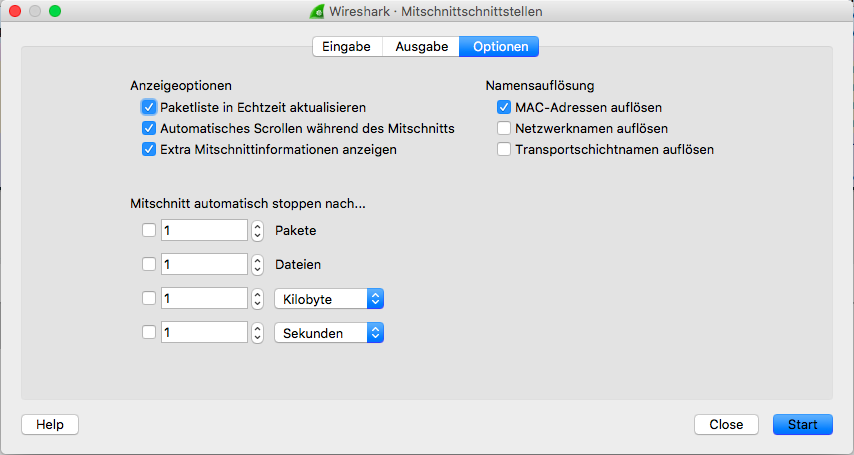
\includegraphics[width=0.8 \linewidth]{images/w01}
	\caption{Capture Options} \label{ordner}
\end{figure} 
Man kann sich aber unter den Statistiken die bei der Aufzeichnung aufgezeichneten Pakete den prozentualen Anteil der Protokolle anzeigen lassen.
\begin{figure}[H]
	\centering
	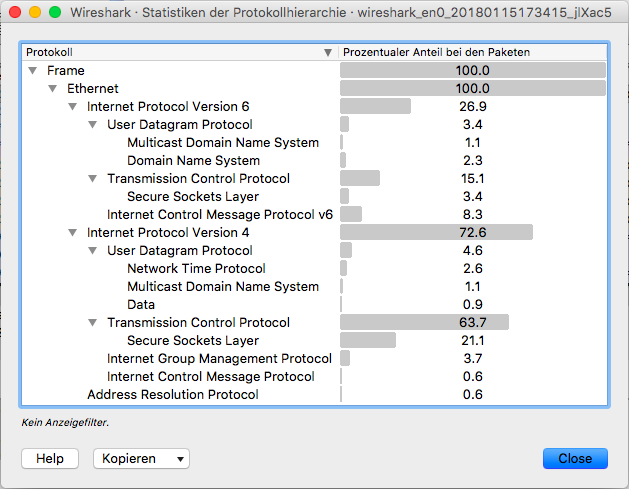
\includegraphics[width=0.7 \linewidth]{images/w02}
	\caption{Protokollhierachie} \label{ordner}
\end{figure} 

\subsubsection{b)}
Für diese Aufgabe erstellen wir einen sogenannten \textit{Mitschnittfilter}, dies geht unter \textbf{Aufzeichnen > Mitschnittfilter}. Um die Aufzeichnung nun damit zu starten wählt man diesen bei der Auszeichnung aus. 
\begin{figure}[H]
	\begin{minipage}[b]{.5 \linewidth}
		\centering
		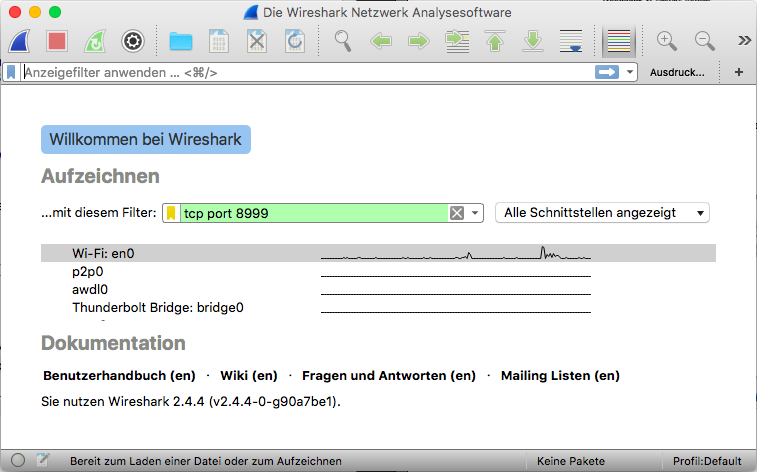
\includegraphics[width=.95 \linewidth]{images/w03}
	\end{minipage}
	\begin{minipage}[b]{.5 \linewidth}
		\centering
		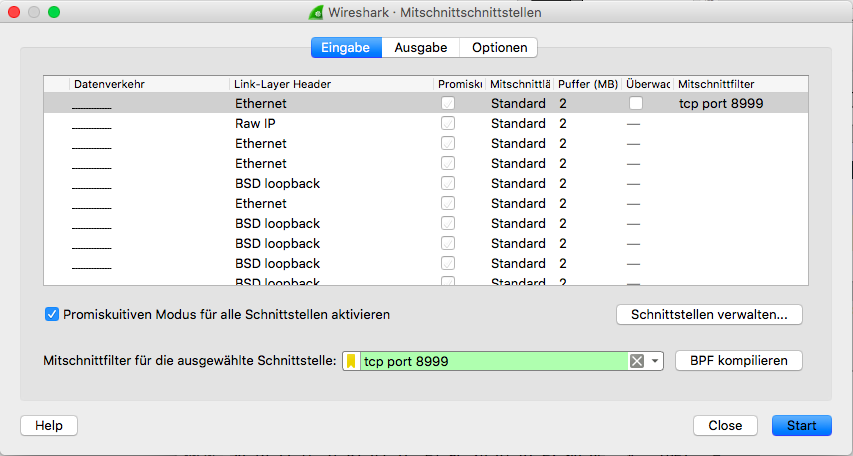
\includegraphics[width=.95 \linewidth]{images/w04}
	\end{minipage}
	\caption{Einstellung des Mitschnittfilters}
\end{figure}

\subsubsection{c)}
Wir nutzen für diese Aufgabe das Programm welches über das UDP-Protokoll arbeitet, da wir aber lokal arbeiten müssen wir über einen sogenannten \textit{Loopback} arbeiten.
\begin{figure}[H]
	\centering
	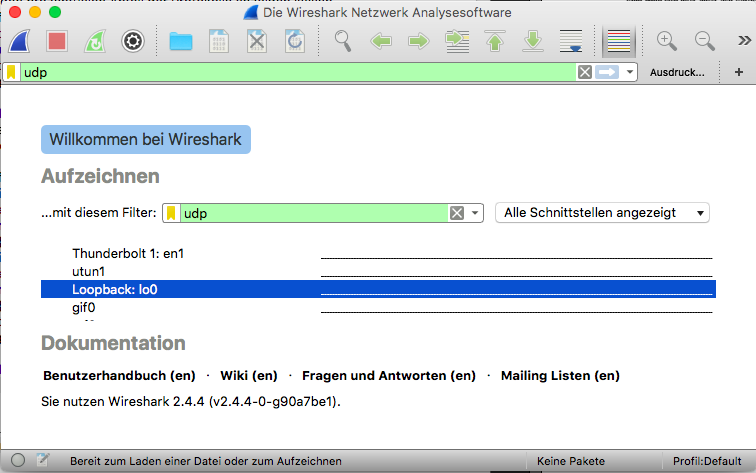
\includegraphics[width=0.7 \linewidth]{images/w05}
	\caption{Loopback} \label{ordner}
\end{figure} 

\subsubsection{d)}
Wir analysieren nun den die Anfrage vom Client zum Server und seine Reaktion darauf. Als erstes stellen wir fest, wie wir erfahren was der Client schickt und was der Server schickt. 
\begin{figure}[H]
	\centering
	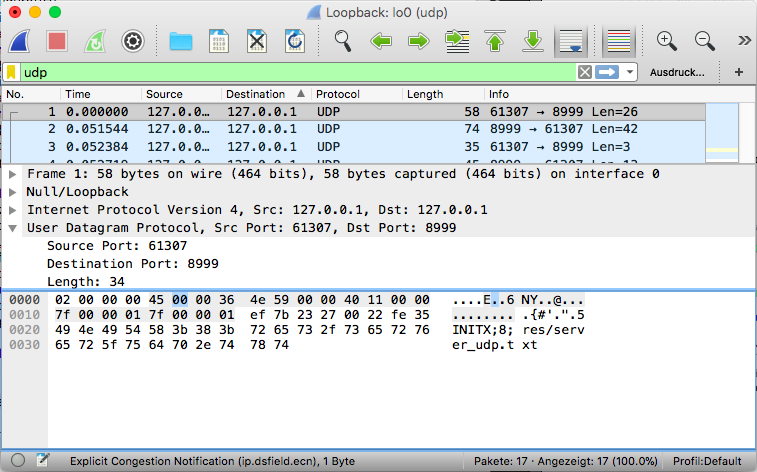
\includegraphics[width=0.6 \linewidth]{images/w06}
	\caption{Erste Nachricht} \label{ordner}
\end{figure} 
Hier erkennen wir das es der Client ist daran das der \textit{Source Port} nicht 8999 ist sondern das ist Ziel ist und wir wissen das der Server auf 8999 arbeitet. Ebenfalls sehen wir das der Client, \textbf{INITX} sendet, die gewollte Größe des Chunks und den Dateinamen mit sendet. 
\begin{figure}[H]
	\centering
	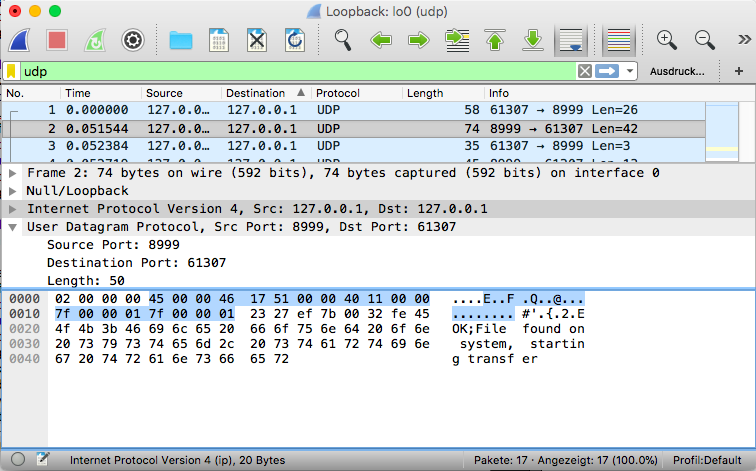
\includegraphics[width=0.6 \linewidth]{images/w07}
	\caption{Server Response} \label{ordner}
\end{figure} 
Hier erkennen wir den Server daran das der \textit{Source Port} 8999 ist. Wir sehen noch das was der Server zurück gibt. Er gibt ein \textit{OK} zurück und eine Nachricht für den Client.\\\\Als nächstes Fragt der Client nach die Daten mit einem \textit{GET} und der Server wird ihn diese drauf zusenden.
\begin{figure}[H]
	\begin{minipage}[b]{.5 \linewidth}
		\centering
		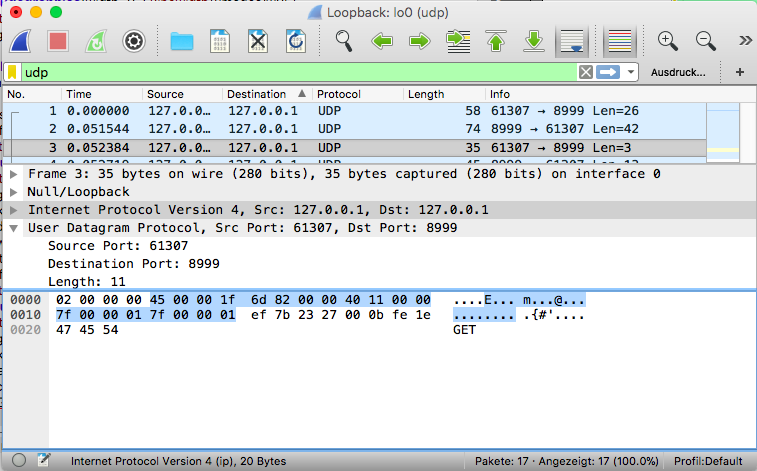
\includegraphics[width=.95 \linewidth]{images/w08}
		\caption{GET-Request des Clients}
	\end{minipage}
	\begin{minipage}[b]{.5 \linewidth}
		\centering
		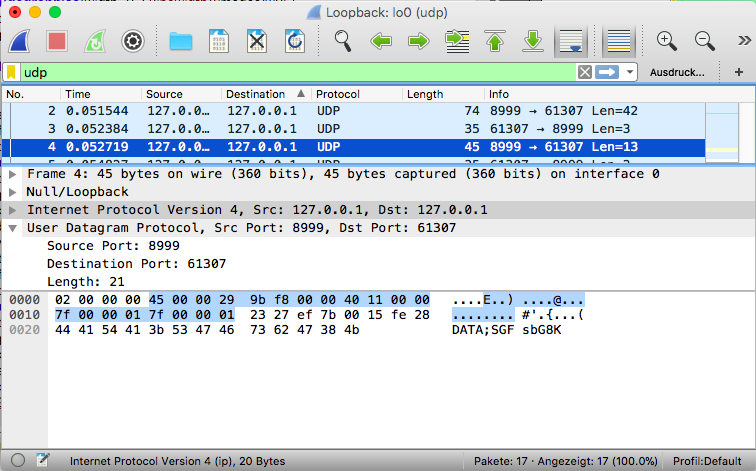
\includegraphics[width=.95 \linewidth]{images/w09}
		\caption{DATA-Response vom Server}
	\end{minipage}
\end{figure}
Der Server sendet ihm die Daten solange zu bis diese fertig gesendet wurden und sendet dann ein \textbf{FINISH}
\begin{figure}[H]
	\centering
	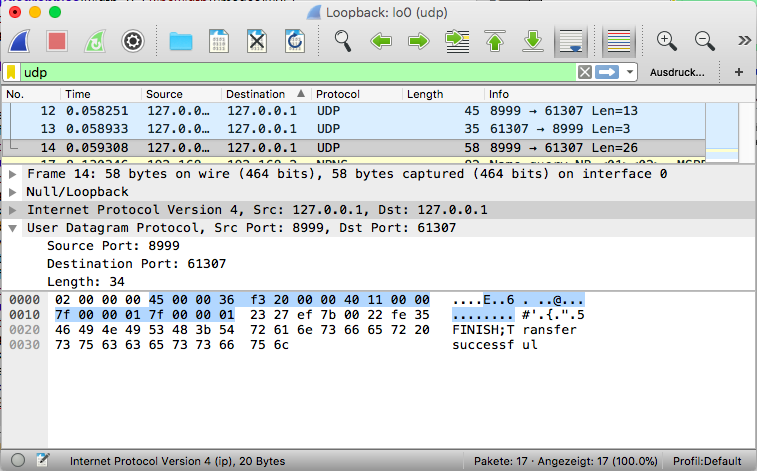
\includegraphics[width=0.6 \linewidth]{images/w10}
	\caption{FINISH-Response} \label{ordner}
\end{figure} 